\documentclass{osa-article}

%% Select the journal you're submitting to
%% oe, boe, ome, osac, osajournal
\journal{oe}
% Key:
% Express journals must have the correct journal selected:
% {oe} Optics Express
% {boe} Biomedical Optics Express
% {ome} Optical Material Express
% {osac} OSAC Continuum
% Other OSA journals may use:
% {osajournal} Applied Optics, Advances in Optics and Photonics, Journal of the Optical Society of America A/B, Optics Letters, Optica, Photonics Research

% Uncomment if submitting to Photonics Research.
% ONLY APPLICABLE FOR \journal{osajournal}
% \setprjcopyright

% Set the article type
\articletype{Research Article}
% Note that article type is not required for Express journals (OE, BOE, OME and OSAC)

\begin{document}

\title{Ultrafast transient absorption measurements of photocarrier dynamics in monolayer and bulk ReSe$_2$}

\author{Jiaqi He,\authormark{1,2,4} Lu Zhang, \authormark{1,4} Dawei He, \authormark{1,5} Yongsheng Wang,\authormark{1,6} Zhiyi He, \authormark{2} and Hui Zhao\authormark{3}}

\address{\authormark{1}Key laboratory of Luminescence and Optical Information, Ministry of education, Institute of Optoelectronic Technology, Beijing Jiaotong University, Beijing 100044, China}

\address{\authormark{2}Guangxi Colleges and Universities Key Laboratory of Microwave and Optical Wave-applied Technology, Guilin 541004, China}

\address{\authormark{3}Department of Physics and Astronomy, The University of Kansas, Lawrence, Kansas 66045, United States}

\address{\authormark{4}These authors contributed equally to this work}

\address{\authormark{5}dwhe@bjtu.edu.cn}

\address{\authormark{6}yshwang@bjtu.edu.cn}
 %% email address is required

% \homepage{http:...} %% author's URL, if desired

%%%%%%%%%%%%%%%%%%% abstract %%%%%%%%%%%%%%%%
%% [use \begin{abstract*}...\end{abstract*} if exempt from copyright]

\begin{abstract}
Recently, transition metal dichalcogenides have been extensively studied as new functional materials for electronic and optoelectronic applications. Most initial efforts have been focused on several members of this material family with 2$H$ lattice structure. ReSe$_2$ as a less-study transition metal dichalcogenide has gained significant momentum due to its 1$T$ lattice structure and in-plane anisotropic electronic and optical properties. Extensive efforts have shown its promising future as a novel material for optoelectronics. However, little was known about the photocarrier dynamics in this material. Here we report the first transient absorption measurement of photocarrier dynamics in ReSe$_2$ bulk and monolayer sample in reflection geometry. We observed ultrafast thermalization and relaxation of hot carriers in bulk ReSe$_2$, and obtained a photocarrier lifetime on the order of 80 ps and decreases slightly with increasing the carrier density. Pronounced anisotropic response of differential reflection was observed. We also studied monolayer ReSe$_2$ samples obtained by chemical vapor deposition and deduced a photocarrier lifetime on the order of 10 ps. These results provide fundamental information for using this material in various optoelectronic devices.
\end{abstract}


\begin{thebibliography}{1}
\newcommand{\enquote}[1]{``#1''}

\bibitem{ssc61531}
G.~Leicht, H.~Berger, and F.~Levy, \enquote{The growth of n-type and p-type
  {ReS$_2$} and {ReSe$_2$} single-crystals and their electrical pproperties,}
  Solid State Commun. \textbf{61}, 531--534 (1987).

\bibitem{b5515608}
C.~H. Ho, P.~C. Liao, Y.~S. Huang, and K.~K. Tiong, \enquote{Temperature
  dependence of energies and broadening parameters of the band-edge excitons of
  {ReS$_2$ and ReSe$_2$},} Phys. Rev. B \textbf{55}, 15608--15613 (1997).

\bibitem{jap816380}
C.~H. Ho, P.~C. Liao, Y.~S. Huang, T.~R. Yang, and K.~K. Tiong,
  \enquote{Optical absorption of {ReS$_2$ and ReSe$_2$} single crystals,} J.
  Appl. Phys. \textbf{81}, 6380--6383 (1997).

\bibitem{b5816130}
C.~H. Ho, Y.~S. Huang, K.~K. Tiong, and P.~C. Liao, \enquote{Absorption-edge
  anisotropy in {ReS$_2$} and {ReSe$_2$} layered semiconductors,} Phys. Rev. B
  \textbf{58}, 16130--16135 (1998).

\bibitem{b6015766}
C.~H. Ho, Y.~S. Huang, J.~L. Chen, T.~E. Dann, and K.~K. Tiong,
  \enquote{Electronic structure of {ReS$_2$ and ReSe$_2$} from first-principles
  calculations, photoelectron spectroscopy, and electrolyte
  electroreflectance,} Phys. Rev. B \textbf{60}, 15766--15771 (1999).

\bibitem{jpcm94411}
C.~M. Fang, G.~A. Wiegers, C.~Haas, and {R. A. de Groot}, \enquote{Electronic
  structures of {ReS$_2$, ReSe$_2$ and TcS$_2$} in the real and the
  hypothetical undistorted structures,} J. Phys.: Condens. Matter \textbf{9},
  4411--4424 (1997).

\bibitem{ssc111635}
K.~K. Tiong, C.~H. Ho, and Y.~S. Huang, \enquote{The electrical transport
  properties of {ReS$_2$ and ReSe$_2$} layered crystals,} Solid State Commun.
  \textbf{111}, 635--640 (1999).

\bibitem{n522274}
E.~Gibney, \enquote{The super materials that could trump graphene,} Nature
  \textbf{522}, 274--276 (2015).

\bibitem{nn7699}
Q.~H. Wang, K.~Kalantar-Zadeh, A.~Kis, J.~N. Coleman, and M.~S. Strano,
  \enquote{Electronics and optoelectronics of two-dimensional transition metal
  dichalcogenides,} Nat. Nanotechnol. \textbf{7}, 699--712 (2012).

\bibitem{2dm3042001}
Z.~Lin, A.~McCreary, N.~Briggs, S.~Subramanian, K.~H. Zhang, Y.~F. Sun, X.~F.
  Li, N.~J. Borys, H.~T. Yuan, S.~K. Fullerton-Shirey, A.~Chernikov, H.~Zhao,
  S.~McDonnell, A.~M. Lindenberg, K.~Xiao, B.~J. LeRoy, M.~Drndic, J.~C.~M.
  Hwang, J.~Park, M.~Chhowalla, R.~E. Schaak, A.~Javey, M.~C. Hersam,
  J.~Robinson, and M.~Terrones, \enquote{{2D} materials advances: From large
  scale synthesis and controlled heterostructures to improved characterization
  techniques, defects and applications,} 2D Mater. \textbf{3}, 042001 (2016).

\bibitem{nl101271}
A.~Splendiani, L.~Sun, Y.~Zhang, T.~Li, J.~Kim, C.~Y. Chim, G.~Galli, and
  F.~Wang, \enquote{Emerging photoluminescence in monolayer {MoS$_2$},} Nano
  Lett. \textbf{10}, 1271--1275 (2010).

\bibitem{l105136805}
K.~F. Mak, C.~Lee, J.~Hone, J.~Shan, and T.~F. Heinz, \enquote{Atomically thin
  {MoS$_2$}: A new direct-gap semiconductor,} Phys. Rev. Lett. \textbf{105},
  136805 (2010).

\bibitem{b87161403}
N.~Kumar, S.~Najmaei, Q.~Cui, F.~Ceballos, P.~M. Ajayan, J.~Lou, and H.~Zhao,
  \enquote{Second harmonic microscopy of monolayer {MoS$_{2}$},} Phys. Rev. B
  \textbf{87}, 161403 (2013).

\bibitem{nl133329}
Y.~Li, Y.~Rao, K.~F. Mak, Y.~You, S.~Wang, C.~R. Dean, and T.~F. Heinz,
  \enquote{Probing symmetry properties of few-layer {MoS$_2$} and {h-BN} by
  optical second-harmonic generation,} Nano Lett. \textbf{13}, 3329--3333
  (2013).

\bibitem{l113076802}
A.~Chernikov, T.~C. Berkelbach, H.~M. Hill, A.~Rigosi, Y.~L. Li, O.~B. Aslan,
  D.~R. Reichman, M.~S. Hybertsen, and T.~F. Heinz, \enquote{Exciton binding
  energy and nonhydrogenic {R}ydberg series in monolayer {WS$_2$},} Phys. Rev.
  Lett. \textbf{113}, 076802 (2014).

\bibitem{l113026803}
K.~He, N.~Kumar, L.~Zhao, Z.~Wang, K.~F. Mak, H.~Zhao, and J.~Shan,
  \enquote{Tightly bound excitons in monolayer {WSe$_2$},} Phys. Rev. Lett.
  \textbf{113}, 026803 (2014).

\bibitem{s3401311}
L.~Britnell, R.~M. Ribeiro, A.~Eckmann, R.~Jalil, B.~D. Belle, A.~Mishchenko,
  Y.-J. Kim, R.~V. Gorbachev, T.~Georgiou, S.~V. Morozov, A.~N. Grigorenko,
  A.~K. Geim, C.~Casiraghi, A.~H.~C. Neto, and K.~S. Novoselov, \enquote{Strong
  light-matter interactions in heterostructures of atomically thin films,}
  Science \textbf{340}, 1311--1314 (2013).

\bibitem{apl105201905}
H.-L. Liu, C.-C. Shen, S.-H. Su, C.-L. Hsu, M.-Y. Li, and L.-J. Li,
  \enquote{Optical properties of monolayer transition metal dichalcogenides
  probed by spectroscopic ellipsometry,} Appl. Phys. Lett. \textbf{105}, 201905
  (2014).

\bibitem{nn6147}
B.~Radisavljevic, A.~Radenovic, J.~Brivio, V.~Giacometti, and A.~Kis,
  \enquote{Single-layer {MoS$_2$} transistors,} Nat. Nanotechnol. \textbf{6},
  147--150 (2011).

\bibitem{nm12815}
B.~Radisavljevic and A.~Kis, \enquote{Mobility engineering and a
  metal-insulator transition in monolayer {MoS$_2$},} Nat. Mater. \textbf{12},
  815--820 (2013).

\bibitem{nl124674}
H.~Wang, L.~L. Yu, Y.~H. Lee, Y.~M. Shi, A.~Hsu, M.~L. Chin, L.~J. Li,
  M.~Dubey, J.~Kong, and T.~Palacios, \enquote{Integrated circuits based on
  bilayer {MoS$_2$} transistors,} Nano Lett. \textbf{12}, 4674--4680 (2012).

\bibitem{nn9262}
B.~W.~H. Baugher, H.~O.~H. Churchill, Y.~Yang, and P.~Jarillo-Herrero,
  \enquote{Optoelectronic devices based on electrically tunable p-n diodes in a
  monolayer dichalcogenide,} Nat. Nanotechnol. \textbf{9}, 262--267 (2014).

\bibitem{s344725}
Y.~J. Zhang, T.~Oka, R.~Suzuki, J.~T. Ye, and Y.~Iwasa, \enquote{Electrically
  switchable chiral light-emitting transistor,} Science \textbf{344}, 725--728
  (2014).

\bibitem{nn9268}
J.~S. Ross, P.~Klement, A.~M. Jones, N.~J. Ghimire, J.~Yan, D.~G. Mandrus,
  T.~Taniguchi, K.~Watanabe, K.~Kitamura, W.~Yao, D.~H. Cobden, and X.~Xu,
  \enquote{Electrically tunable excitonic light-emitting diodes based on
  monolayer {WSe$_2$} p-n junctions,} Nat. Nanotechnol. \textbf{9}, 268--274
  (2014).

\bibitem{nn9257}
A.~Pospischil, M.~M. Furchi, and T.~Mueller, \enquote{Solar-energy conversion
  and light emission in an atomic monolayer p-n diode,} Nat. Nanotechnol.
  \textbf{9}, 257--261 (2014).

\bibitem{nanoscale67226}
S.~Yang, S.~Tongay, Y.~Li, Q.~Yue, J.~B. Xia, S.~S. Li, J.~Li, and S.~H. Wei,
  \enquote{Layer-dependent electrical and optoelectronic responses of
  {ReSe$_2$} nanosheet transistors,} Nanoscale \textbf{6}, 7226--7231 (2014).

\bibitem{acsnano811154}
D.~Wolverson, S.~Crampin, A.~S. Kazemi, A.~Ilie, and S.~J. Bending,
  \enquote{Raman spectra of monolayer, few-layer, and bulk {ReSe$_2$}: An
  anisotropic layered semiconductor,} ACS Nano \textbf{8}, 11154--11164 (2014).

\bibitem{nl151660}
S.~X. Yang, C.~Wang, H.~Sahin, H.~Chen, Y.~Li, S.~S. Li, A.~Suslu, F.~M.
  Peeters, Q.~Liu, J.~B. Li, and S.~Tongay, \enquote{Tuning the optical,
  magnetic, and electrical properties of {ReSe$_2$} by nanoscale strain
  engineering,} Nano Lett. \textbf{15}, 1660--1666 (2015).

\bibitem{nr83651}
H.~Zhao, J.~B. Wu, H.~X. Zhong, Q.~S. Guo, X.~M. Wang, F.~N. Xia, L.~Yang,
  P.~H. Tan, and H.~Wang, \enquote{Interlayer interactions in anisotropic
  atomically thin rhenium diselenide,} Nano Res. \textbf{8}, 3651--3661 (2015).

\bibitem{b96165418}
H.~F. Wang, E.~F. Liu, Y.~Wang, B.~Wan, C.~H. Ho, F.~Miao, and X.~G. Wan,
  \enquote{Cleavage tendency of anisotropic two-dimensional materials: {ReX$_2$
  (X = S,Se)} and {WTe$_2$},} Phys. Rev. B \textbf{96}, 165418 (2017).

\bibitem{nl173202}
A.~Arora, J.~Noky, M.~Druppel, B.~Jariwala, T.~Deilmann, R.~Schneider,
  R.~Schmidt, O.~D. Pozo-Zamudio, T.~Stiehm, A.~Bhattacharya, P.~Kruger, S.~M.
  de~Vasconcellos, M.~Rohlfing, and R.~Bratschitsch, \enquote{Highly
  anisotropic in-plane excitons in atomically thin and bulklike
  {1$T$-ReSe$_2$},} Nano Lett. \textbf{17}, 3202--3207 (2017).

\bibitem{am288296}
M.~Hafeez, L.~Gan, H.~Q. Li, Y.~Ma, and T.~Y. Zhai, \enquote{Chemical vapor
  deposition synthesis of ultrathin hexagonal {ReSe$_2$} flakes for anisotropic
  raman property and optoelectronic application,} Adv. Mater. \textbf{28},
  8296--8301 (2016).

\bibitem{nr102732}
F.~F. Cui, X.~B. Li, Q.~L. Feng, J.~B. Yin, L.~Zhou, D.~Y. Liu, K.~Q. Liu,
  X.~X. He, X.~Liang, S.~Z. Liu, Z.~B. Lei, Z.~H. Liu, H.~L. Peng, J.~Zhang,
  J.~Kong, and H.~Xu, \enquote{Epitaxial growth of large-area and highly
  crystalline anisotropic {ReSe$_2$} atomic layer,} Nano Res. \textbf{10},
  2732--2742 (2017).

\bibitem{b92115438}
H.~X. Zhong, S.~Y. Gao, J.~J. Shi, and L.~Yang, \enquote{Quasiparticle band
  gaps, excitonic effects, and anisotropic optical properties of the monolayer
  distorted {1$T$} diamond-chain structures {ReS$_2$} and {ReSe$_2$},} Phys.
  Rev. B \textbf{92}, 115438 (2015).

\bibitem{am286711}
S.~H. Jo, H.~Y. Park, D.~H. Kang, J.~Shim, J.~Jeon, S.~Choi, M.~Kim, Y.~Park,
  J.~Lee, Y.~J. Song, S.~Lee, and J.~H. Park, \enquote{Broad detection range
  rhenium diselenide photodetector enhanced by (3-aminopropyl)triethoxysilane
  and triphenylphosphine treatment,} Adv. Mater. \textbf{28}, 6711 (2016).

\bibitem{acsnano102752}
E.~Lorchat, G.~Froehlicher, and S.~Berciaud, \enquote{Splitting of interlayer
  shear modes and photon energy dependent anisotropic raman response in n-layer
  {ReSe$_21$} and {ReS$_2$},} ACS Nano \textbf{10}, 2752--2760 (2016).

\bibitem{acsnano108067}
E.~Z. Zhang, P.~Wang, Z.~Li, H.~F. Wang, C.~Y. Song, C.~Huang, Z.~G. Chen,
  L.~Yang, K.~T. Zhang, S.~H. Lu, W.~Y. Wang, S.~S. Liu, H.~H. Fang, X.~H.
  Zhou, H.~G. Yang, J.~Zou, X.~G. Wan, P.~Zhou, W.~D. Hu, and F.~X. Xiu,
  \enquote{Tunable ambipolar polarization-sensitive photodetectors based on
  high-anisotropy {ReSe$_2$} nanosheets,} ACS Nano \textbf{10}, 8067--8077
  (2016).

\bibitem{nr9507}
X.~T. Wang, L.~Huang, Y.~T. Peng, N.~J. Huo, K.~D. Wu, C.~X. Xia, Z.~M. Wei,
  S.~Tongay, and J.~B. Li, \enquote{Enhanced rectification, transport property
  and photocurrent generation of multilayer {ReSe$_2$/MoS$_2$ p-n}
  heterojunctions,} Nano Res. \textbf{9}, 507--516 (2016).

\bibitem{aplm5076101}
A.~J. Cho, S.~D. Namgung, H.~Kim, and J.~Y. Kwon, \enquote{Electric and
  photovoltaic characteristics of a multi-layer {ReS$_2$/ReSe$_2$}
  heterostructure,} APL Mater. \textbf{5}, 076101 (2017).

\bibitem{nl161381}
L.~Hart, S.~Dale, S.~Hoye, J.~L. Webb, and D.~Wolverson, \enquote{Rhenium
  dichalcogenides: Layered semiconductors with two vertical orientations,} Nano
  Lett. \textbf{16}, 1381--1386 (2016).

\bibitem{s42004}
S.~Jiang, M.~Hong, W.~Wei, L.~Zhao, N.~Zhang, Z.~Zhang, P.~Yang, N.~Gao, X.~Zhou, C.~Xie, J.~Shi, Y.~Huan, L.~Tong, J.~Zhao, Q.~Zhang, Q.~Fu, and Y.~Zhang
  \enquote{Direct synthesis and in situ characterization of monolayer parallelogrammic rhenium diselenide on gold foil,} Chem. Commun.
  \textbf{1}, 17 (2018).
  
\bibitem{b86045406}
R.~Wang, B.~A. Ruzicka, N.~Kumar, M.~Z. Bellus, H.-Y. Chiu, and H.~Zhao,
  \enquote{Ultrafast and spatially resolved studies of charge carriers in
  atomically thin molybdenum disulfide,} Phys. Rev. B \textbf{86}, 045406
  (2012).

\bibitem{acsnano82970}
Q.~Cui, F.~Ceballos, N.~Kumar, and H.~Zhao, \enquote{Transient absorption
  microscopy of monolayer and bulk {WSe$_2$},} ACS Nano \textbf{8}, 2970--2976
  (2014).

\bibitem{afm271604509}
F.~Ceballos and H.~Zhao, \enquote{Ultrafast laser spectroscopy of
  two-dimensional materials beyond graphene,} Adv. Funct. Mater. \textbf{27},
  1604509 (2017).

\bibitem{jssc51170}
J.~V. Marzik, R.~Kershaw, K.~Dwight, and A.~Wold, \enquote{Photoelectronic
  properties of {ReS$_2$ and ReSe$_2$} single crystals,} J. Solid. State. Chem.
  \textbf{51}, 170--175 (1984).

\bibitem{jap113133702}
N.~Kumar, J.~He, D.~He, Y.~Wang, and H.~Zhao, \enquote{Charge carrier dynamics
  in bulk {MoS$_2$} crystal studied by transient absorption microscopy,} J. of
  Appl. Phys. \textbf{113}, 133702 (2013).

\bibitem{nanoscale64915}
N.~Kumar, Q.~Cui, F.~Ceballos, D.~He, Y.~Wang, and H.~Zhao, \enquote{Exciton
  diffusion in monolayer and bulk {MoSe$_2$},} Nanoscale \textbf{6}, 4915--4919
  (2014).

\bibitem{nanoscale79526}
J.~He, D.~He, Y.~Wang, Q.~Cui, F.~Ceballos, and H.~Zhao,
  \enquote{Spatiotemporal dynamics of excitons in monolayer and bulk WS$_2$,}
  Nanoscale \textbf{7}, 9526 (2015).

\bibitem{b89125427}
N.~Kumar, Q.~Cui, F.~Ceballos, D.~He, Y.~Wang, and H.~Zhao,
  \enquote{Exciton-exciton annihilation in {MoSe$_2$} monolayers,} Phys. Rev. B
  \textbf{89}, 125427 (2014).


\end{thebibliography}
%%%%%%%%%%%%%%%%%%%%%%%%%%  body  %%%%%%%%%%%%%%%%%%%%%%%%%%
\section{Introduction}
ReSe$_2$ is an important type of layered transition metal dichalcogenide (TMD). Several decades ago, high-quality ReSe$_2$ crystals have been grown by chemical vapor transport \cite{ssc61531,b5515608}. Piezoreflectance \cite{b5515608} and optical absorption measurements \cite{jap816380} revealed a direct bandgap in the range of 1.2 - 1.3 eV at room temperature, with an exciton binding energy of 22 meV \cite{b5515608}. Since its indirect bandgap is smaller than the direct one \cite{b5816130}, bulk ReS$_2$ is an indirect semiconductor. Results of first-principle calculations, ultraviolet photoelectron spectroscopy, and electrolyte electroreflectance also confirmed its indirect nature \cite{b6015766,jpcm94411}. As a layered material with distorted 1$T$ structure, the charge transport property of ReSe$_2$ is highly anisotropic. The in-plane resistivity is about 6 orders of magnitude lower than that along the perpendicular direction \cite{ssc111635}. In the plane, the resistivity show a 4-fold anisotropy, with the smaller resistivity occurring along the direction of Re-chains. \cite{ssc111635}. The in-plane Hall mobilities at room temperature are on the order of 20 cm$^2$ V$^{-1}$ s$^{-1}$ \cite{ssc111635}. The bandgap was also found to be anisotropic, with values of 1.17 and 1.20 eV for light polarized parallel and perpendicular to the Re-chains, respectively \cite{b5816130}.

Recently, ReSe$_2$ has regained a lot of interests in the context of two-dimensional (2D) materials. 
These atomically thin materials have drawn significant interests as a new form of nanomaterials \cite{n522274,nn7699,2dm3042001}. Among the 2D materials studied so far, TMDs have been a focused material family. TMDs possess thickness-dependent electronic structures \cite{nl101271,l105136805} and crystal symmetry \cite{b87161403,nl133329}, strong excitonic effects \cite{l113076802,l113026803}, and large optical absorption coefficients \cite{s3401311,apl105201905}. They have shown promising applications in field-effect transistors \cite{nn6147,nm12815}, integrated circuits \cite{nl124674}, solar cells\cite{nn9262}, photodetectors \cite{nn9262}, and light-emitting diodes \cite{s344725,nn9268,nn9257}. However, most studies of 2D TMDs have focused on a few members of this rich family, such as MoS$_2$, MoSe$_2$, WS$_2$, and WSe$_2$ \cite{2dm3042001}. Because these materials have the same 2$H$ lattice structure, their properties are also similar to a certain degree. 

Two-dimensional ReSe$_2$ have been suggested as a new 2D TMD of interests, due to its rather unique properties that are originated from its distorted 1$T$ structure with triclinic symmetry  \cite{jpcm94411}. Monolayer (ML) and few-layer ReSe$_2$ have been successfully fabricated by mechanical exfoliation \cite{nanoscale67226,acsnano811154,nl151660,nr83651,b96165418,nl173202}, chemical vapor deposition \cite{am288296}, and epitaxial growth \cite{nr102732}. Some theoretical works suggested that the bandgap of ReSe$_2$ increases with decreasing the thickness, but remains its indirect nature even at ML limit \cite{nanoscale67226,acsnano811154}. However, more studies of density functional theory \cite{nl151660} and many-body perturbation theory \cite{b92115438} showed that ML ReSe$_2$ is a direct semiconductor. Indeed, photoluminescence (PL) of ML ReSe$_2$ peaked at 1.47 eV at room temperature has been observed \cite{nl151660}. Low-temperature PL measurements showed that at 80 K, the PL peak energy changes from 1.32 in ML to 1.27 eV in bulk \cite{nr83651}. Furthermore, the PL yield increases with thickness  \cite{nr83651}, suggesting the lack of an indirect-to-direct transition - a common feature of other TMDs. These latest results appear to challenge the previous understanding that bulk ReSe$_2$ is indirect. In ML form, excitons have large binding energies and rich features, as shown by low-temperature and polarization-resolved PL and transmission spectroscopy \cite{nl173202}.

Significant progress has been made in developing optoelectronic devices with 2D ReSe$_2$. Several groups have reported high-performance photodetectors based on ultrathin ReSe$_2$ \cite{am288296,nr102732}, illustrating the potential of this 2D material for broadband, high-responsivity, and fast-response photodetection applications \cite{am286711}. Furthermore, the in-plane anisotropic lattice dynamics and optical responses, as revealed by PL \cite{nr83651,nl173202} and Raman spectroscopy \cite{acsnano811154,acsnano102752}, can be utilized in polarization-sensitive photodetectors \cite{acsnano108067}. On electronic applications, single-layer ReSe$_2$ field-effect transistors have been demonstrated, with mobilities in the range of 1 to 10 cm$^2$ V$^{-1}$ s$^{-1}$  \cite{nr102732,nanoscale67226} and current on/off ratio up to 10$^5$ \cite{nr102732}. Few-layer-based devices achieved an excellent on/off ratio exceeding 10$^7$ \cite{acsnano108067}. Furthermore, it was shown that the optical, magnetic, and electrical properties of ML ReSe$_2$ are very sensitive to lattice strain \cite{nl151660}, which offers opportunities such as strain-engineered devices or strain sensors. In addition to these potential applications as an individual material, ReSe$_2$ can also be used to fabricate 2D heterostructures. For example, multilayer ReSe$_2$-MoS$_2$ heterostructure with a type-II band alignment can be used for photodetectors \cite{nr9507}; while photovoltaic effect has been observed in multilayer ReSe$_2$-ReS$_2$ heterostructures \cite{aplm5076101}. In this regard, the unique feature that ML ReSe$_2$ is nonsymmetric about $C$2 rotation about an in-plane axis  \cite{nl161381} offers additional freedom to design heterostructures.

So far, little was known about the photocarrier dynamics in ReSe$_2$. However, photocarrier dynamics play an important role in application of semiconductors in optoelectronic devices. For example, the photocarrier lifetime often controls the sensitivity of photodetectors and the energy conversion efficiency of solar cells. Here we report the first time-resolved study of photocarrier dynamics in both bulk and ML ReSe$_2$. By performing transient absorption measurements, we reveal the ultrafast thermalization and relaxation dynamics of photocarriers in bulk ReSe$_2$, and deduced a photocarrier lifetime on the order of 80 ps. We also observed in-plane anisotropic transient absorption response of ReSe$_2$. In monolayer ReSe$_2$ fabricated by chemical vapor depositioin, the photocarrier lifetime is on the order of 10 ps. These results provide fundamental information for using this material in various optoelectronic devices.


\section{Experimental}

ReSe$_2$ has a distorted 1$T$ structure with triclinic symmetry \cite{jpcm94411}. Figs. \ref{fig:sample}(a) and \ref{fig:sample}(b) show a top view and a side view of multilayer ReSe$_2$, respectively. The Re atoms in each layer form diamond chains \cite{jpcm94411}, as indicated by the red lines. In this study, bulk flakes of ReSe$_2$ were mechanically exfoliated from crystals purchased from 2D Semiconductors. A thermal-release adhesive tape was used to transfer flakes from the crystal to a Si substrate with a 300-nm SiO$_2$ top layer. Fig. \ref{fig:sample}(d) shows an optical microscope image of the bulk sample studied. The horizontal (H) and vertical (V) directions in the laboratory frame are labeled. $\theta$ is defined as the angle between H and the long edge of the flake (dashed line). We also studied monolayer ReSe$_2$ samples acquired from 6 Carbon, which are fabricated by chemical vapor deposition and transferred to a Al$_2$O$_3$ substrate, as shown in Fig. \ref{fig:sample}(c). Fig. \ref{fig:sample}(e) shows an atomic force microscope (AFM) image of the ReSe$_2$ monolayer sample. The thickness of the sample is about 1.5 nm. Previous AFM measurements have shown a ReSe$_2$ monolayer thickness of 0.9 nm \cite{s42004}. Since the thickness obtained here is smaller than 1.8 nm, it confirmed that the sample is monolayer and the difference could be attributed to foreign agencies on the surface or under the ReSe$_2$ layer.

\begin{figure}
  \centering
  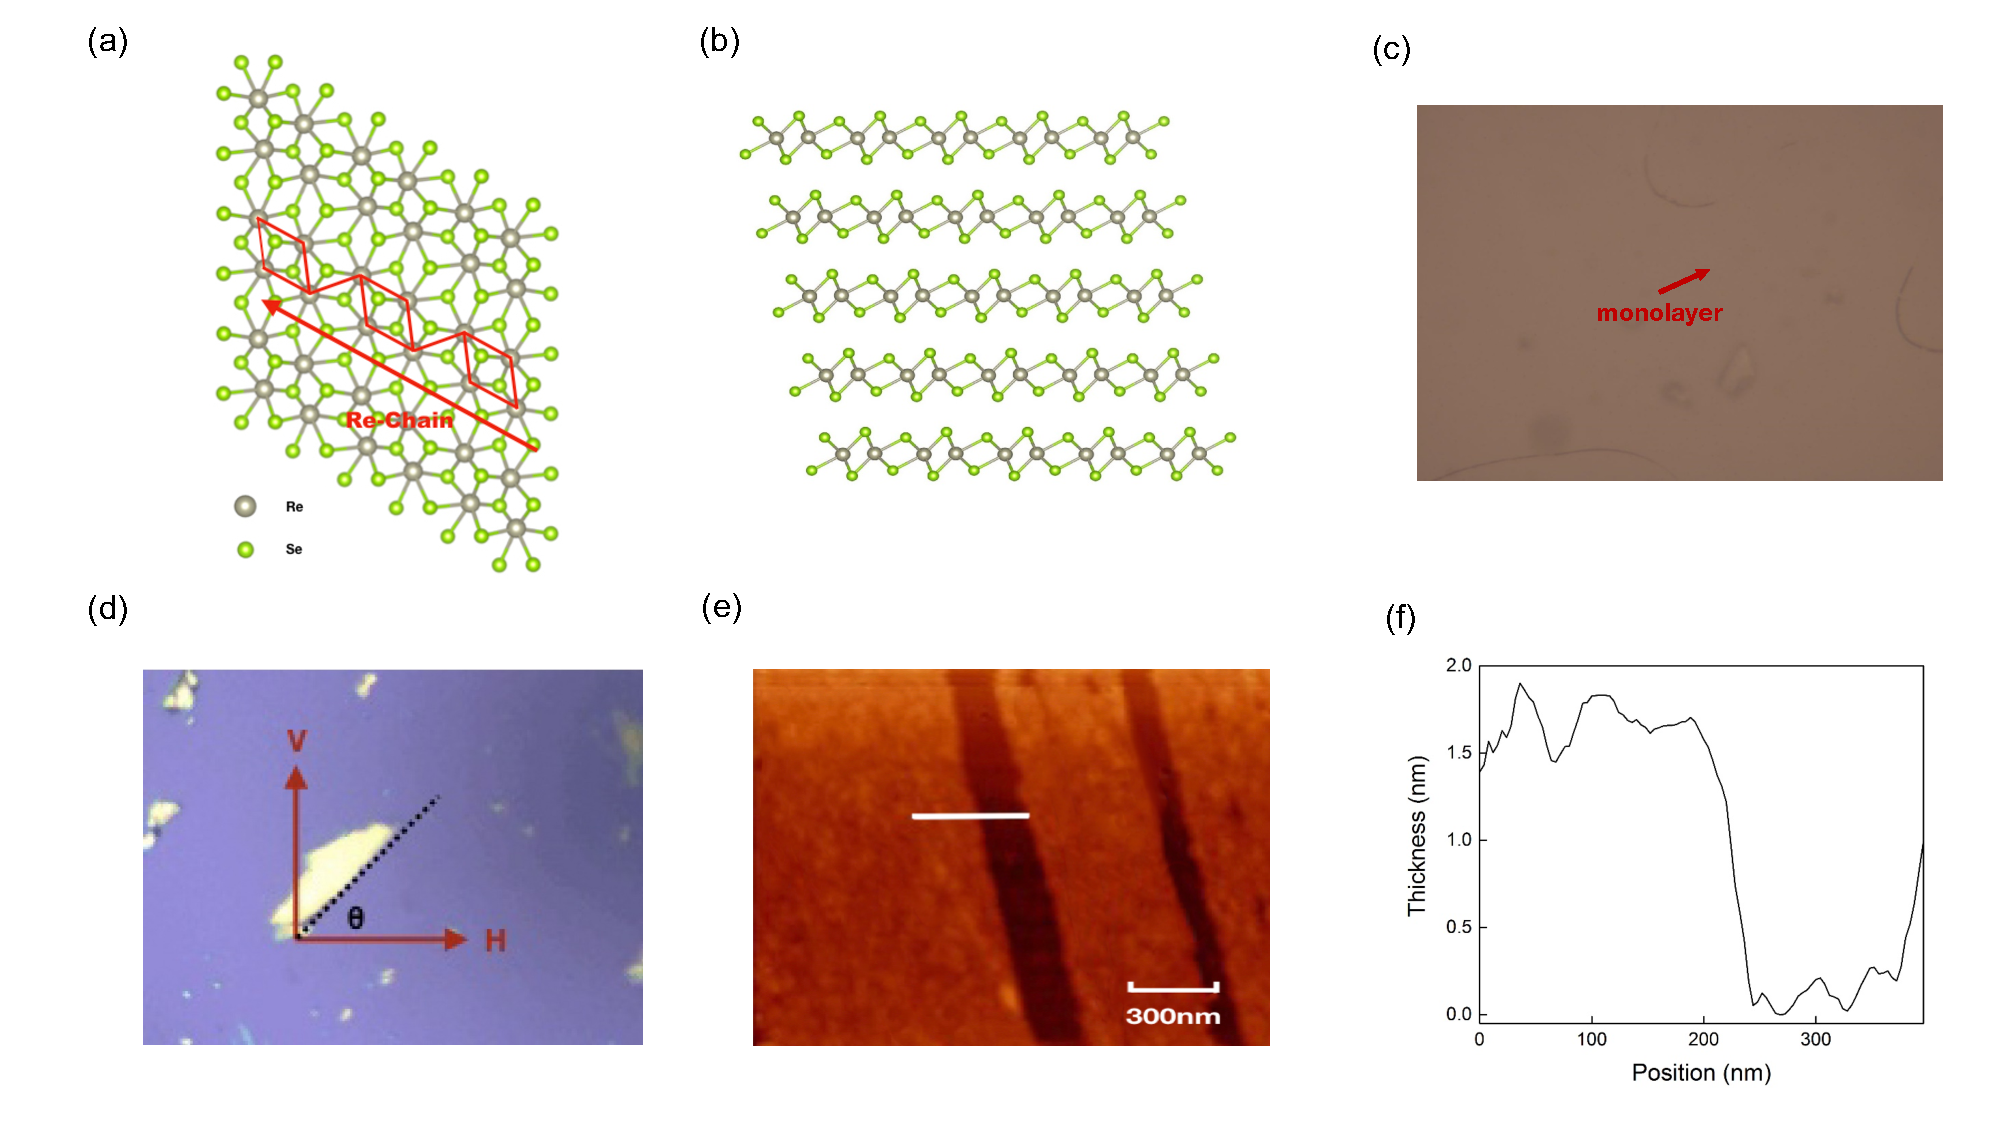
\includegraphics[width=10.5cm]{sample.pdf}
  \caption{(a) Top view of the lattice structure of monolayer ReSe$_2$. (b) Side view of multilayer ReSe$_2$. (c) Optical image of the ReSe$_2$ monolayer sample.(d) Microscope image of the bulk ReSe$_2$ sample studied. The horizontal (H) and vertical (V) directions in the laboratory coordinates are labeled. The angle $\theta$ is between H and the long edge of the flake. (e) Atomic force microscope (AFM) image of the ReSe$_2$ monolayer sample. (f) A line scan of the AFM image shown by the white line in (e).}
    \label{fig:sample}
\end{figure}


Photocarrier dynamics in these samples were studied by a transient absorption technique \cite{b86045406,acsnano82970,afm271604509}. Fig. \ref{fig:setup} shows schematically the differential reflection setup used in this study. A 532-nm diode laser pumps a Ti:sapphire laser, which generates 100-fs pulses with a central wavelength of 820 nm and an average power of about 4 W. A beamsplitter (BS) divides the Ti:sapphire output to two parts. The reflected part (about 90\%) pumps an optical parametric oscillator (OPO) to produce a signal output with a central wavelength of 620 nm, which serves as the pump pulse for the measurements. The rest of the Ti:sapphire output serves directly as the probe pulse.  The two beams were combined with another BS and were focused to the sample through a microscope objective lens. Both beamsplitters before the objective lens have same ratio of 50\% reflected. Since each beam (pump or probe) goes through a half-wave plate and a polarizer to adjust its polarization and power, the ratio of beam splitter has no effect on our results. 
 The sizes of the pump and probe spots are about 1.8 and 2.5 $\mu$m in full width at half maximum (FWHM), respectively. The reflected probe was sent to a silicon photodiode, which output was measured by a lock-in amplifier. A set of filters were used to prevent the pump beam from reaching the photodiode. A mechanical chopper (not shown) was placed in the pump arm to modulate its intensity at about 2 KHz. Since the laser repetition rate is about 80 MHz, there are many pulses during one cycle of the chopper modulation. With this configuration, we can measure the differential reflection of the probe by the sample, which is defined as $\Delta R / R_0 = (R - R_0)/R_0$, where $R$ and $R_0$ are the reflection coefficient of the probe with and without the pump beam, respectively. In the measurement, the differential reflection was measured as a function of the probe delay, which is defined as the arrival time of the probe pulse at the sample position with respect to the pump pulse and was controlled by changing the path length of the probe pulse with a delay stage. All measurements were performed with the sample under ambient condition. 

\begin{figure}
  \centering
  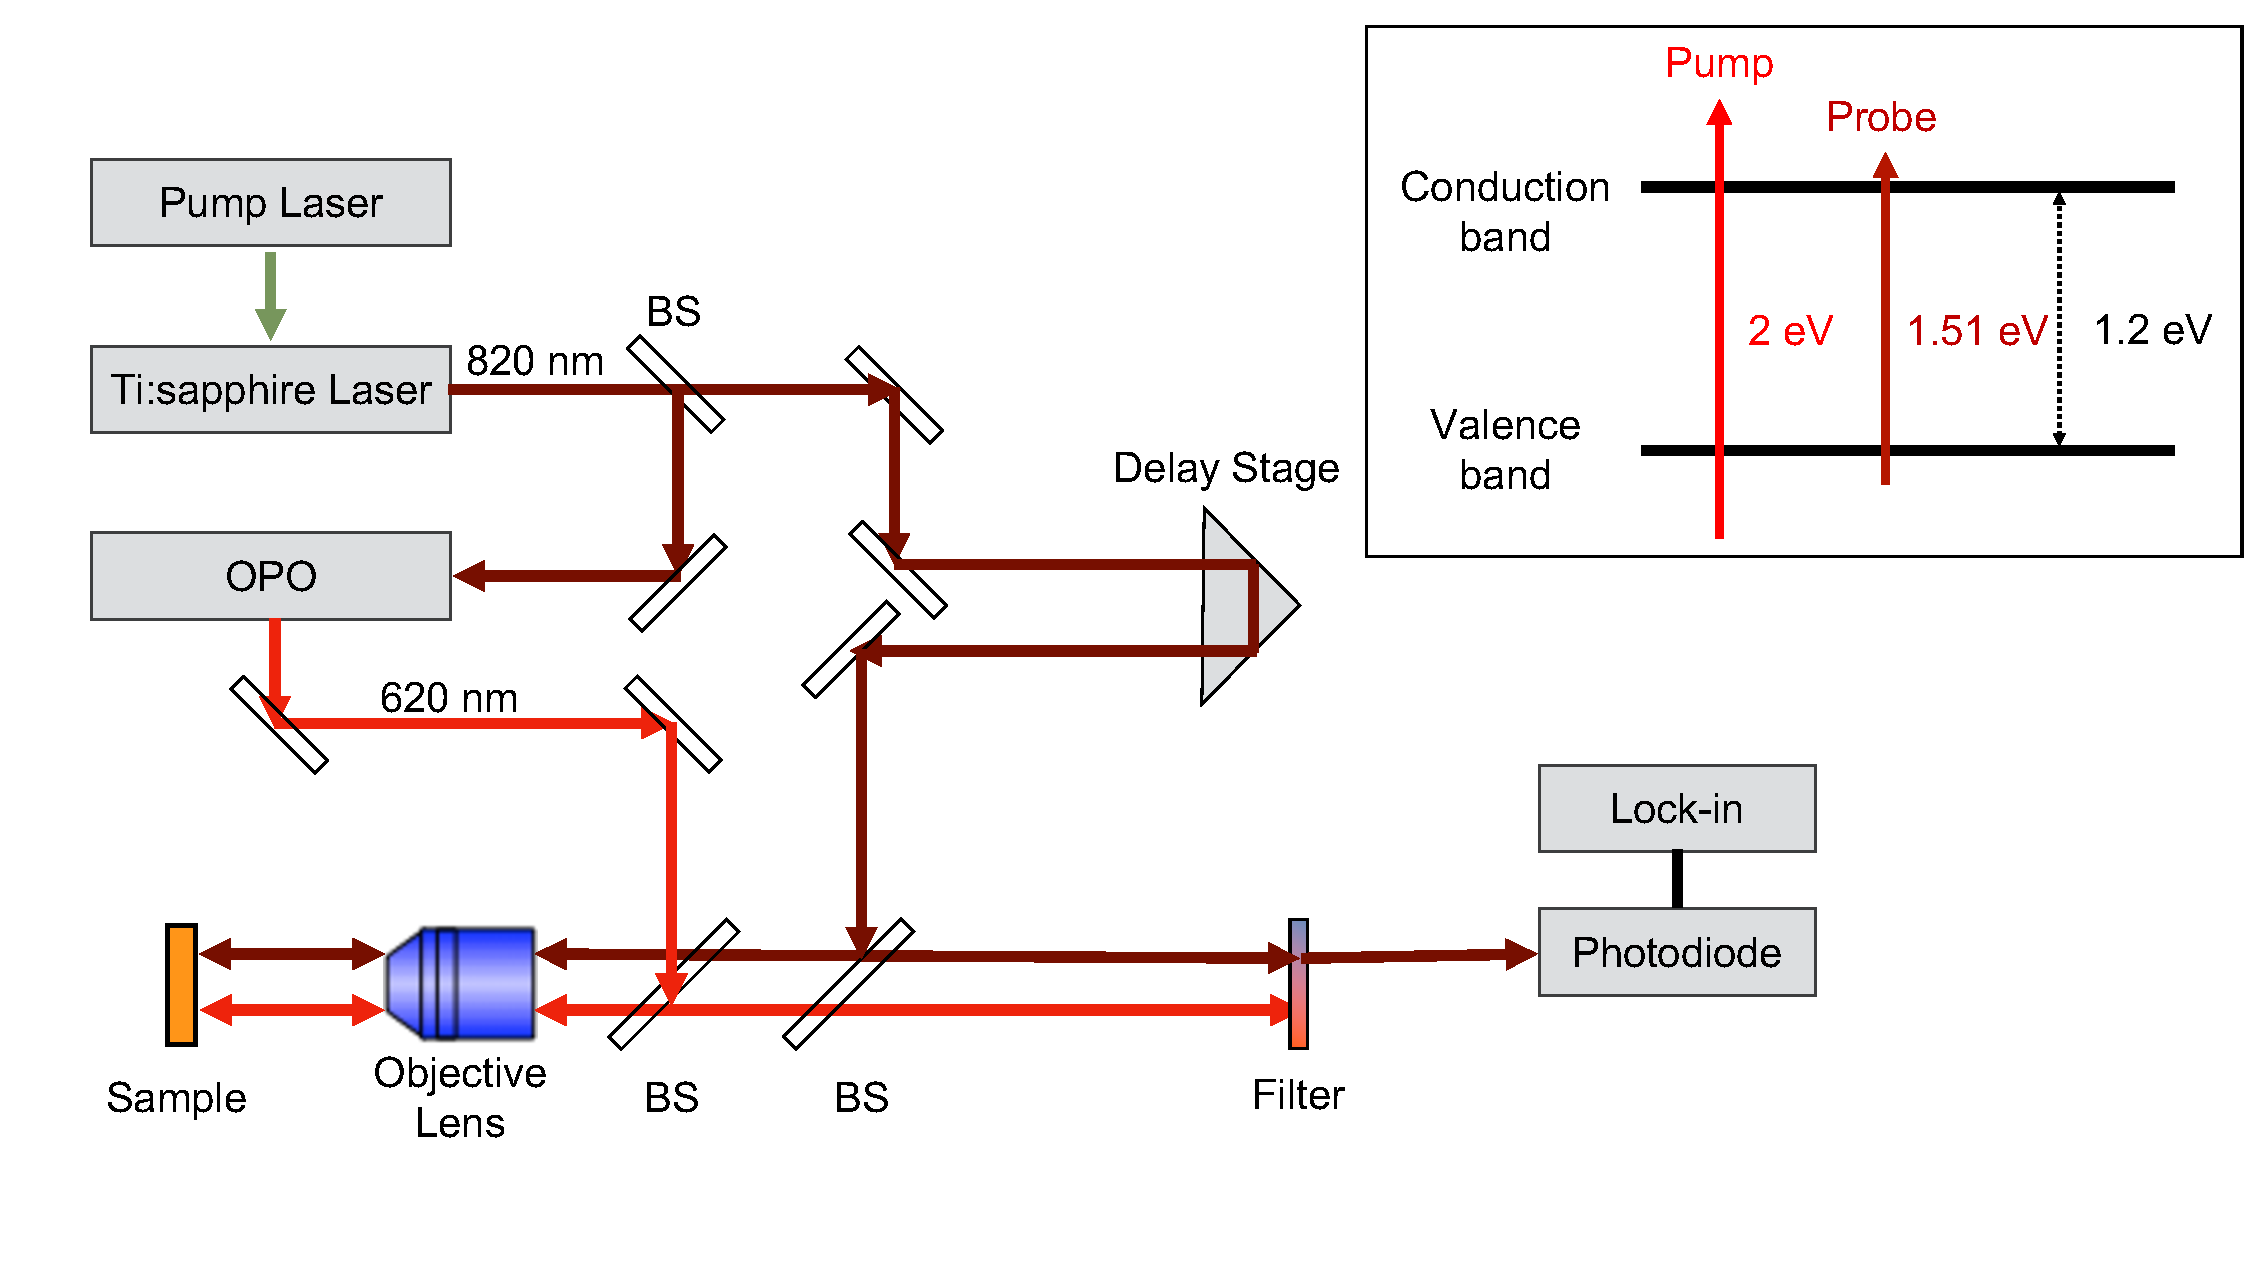
\includegraphics[width=10cm]{setup.pdf}
  \caption{Schematics of the differential reflection setup.The inset showes energy diagram of ReSe$_2$ and pump-probe scheme. }
    \label{fig:setup}
\end{figure}

\section{Results and discussion}

We first studied the bulk sample, with the pump and probe pulses linearly polarized along V and H directions, and with a sample orientation of $\theta = 0^\circ$. The 620-nm pump pulse injects photocarriers {\it via} interband absorption, which dynamics is monitored by the 820-nm probe. Since the direct bandgap of bulk ReSe$_2$ is about 1.2 to 1.3 eV\cite{jap816380}, the probe photon energy of 1.51 eV is about 0.2 - 0.3 eV above the bandgap, while the pump photon energy of about 2 eV is even higher. Figure \ref{fig:bulk}(a) and (b) show examples of the observed signal over a short (a) and long (b) time ranges, respectively. Different symbols correspond to measurements with different values of the pump fluence, as labeled in (b). To estimate the injected carrier density, we used an absorption coefficient \cite{jssc51170} of 2 $\times$ 10$^7$ m$^{-1}$ and found that a fluence of 1 $\mu$J cm$^{-2}$ injects a peak carrier density of about 1.4 $\times$ 10$^9$ cm$^{-3}$ at the surface of the sample.

\begin{figure}
  \centering
  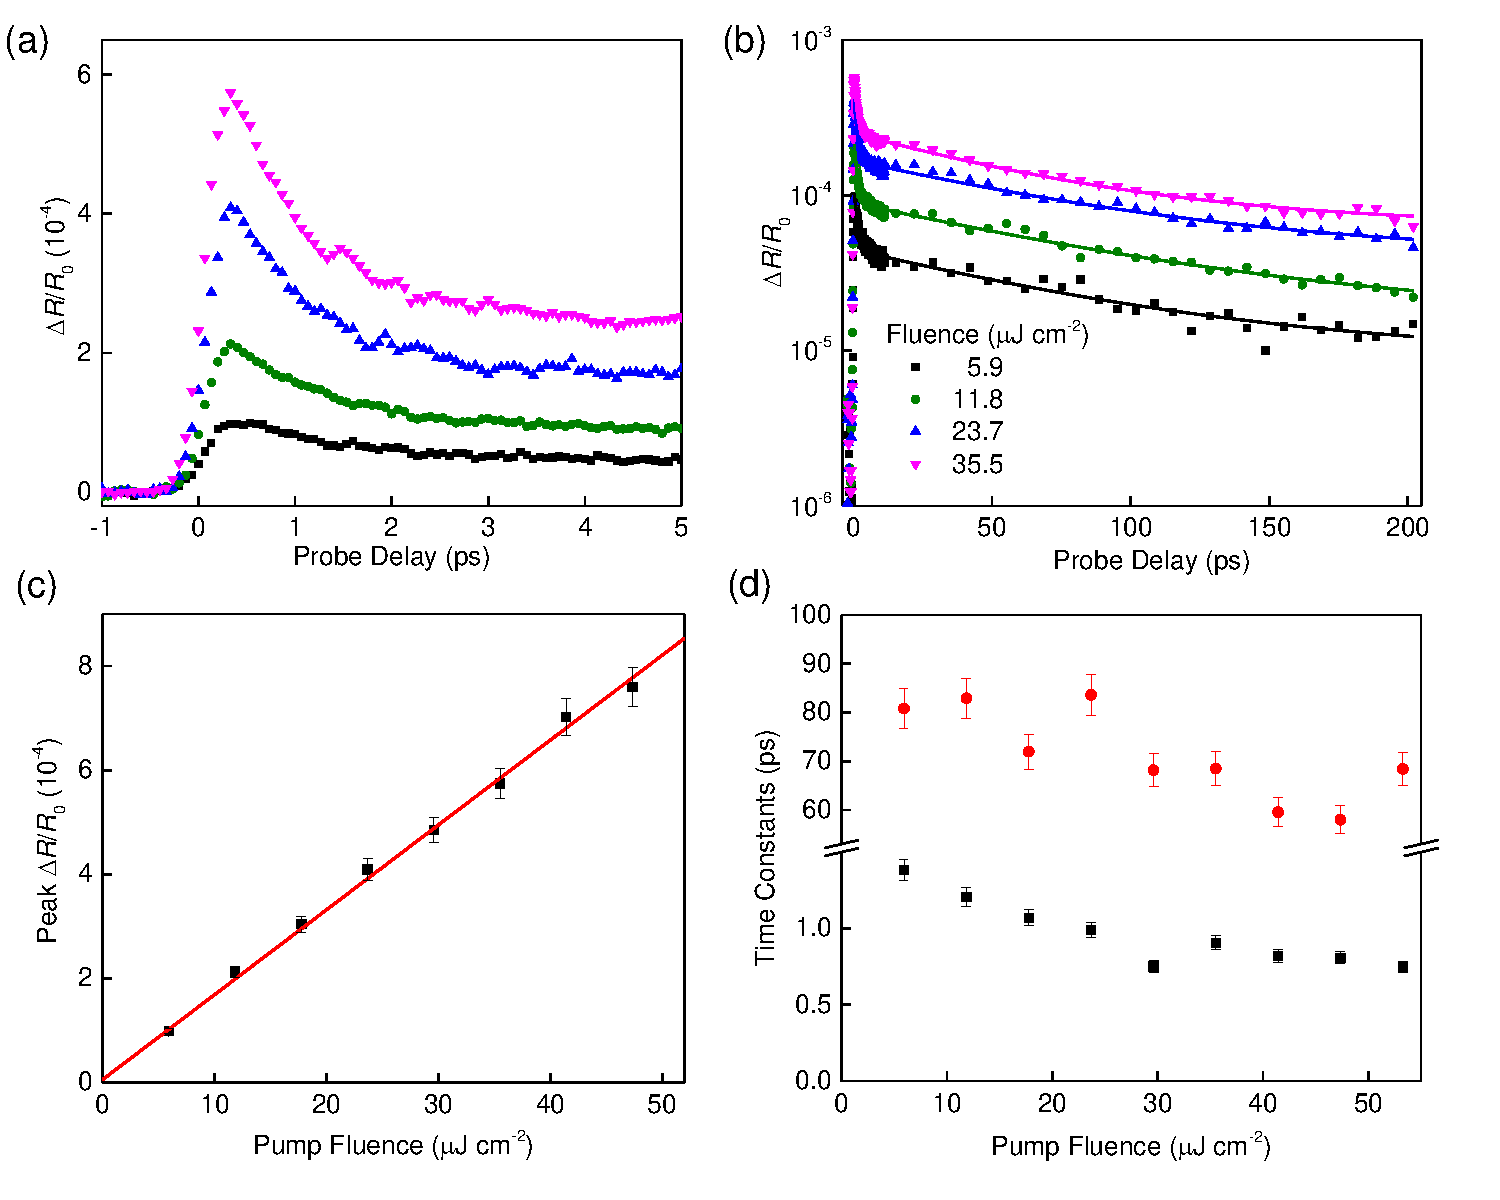
\includegraphics[width=12cm]{bulk.pdf}
  \caption{Differential reflection signal of bulk ReSe$_2$ measured with a 620-nm pump and an 820-nm probe pulses for a short time range (a) and a long time range (b), respectively. Different symbols represent results with different values of the pump fluence, as labeled in (b). (c) shows the peak signal as a function of the pump fluence. (d) shows the two time constants deduced from fits.}
    \label{fig:bulk}
\end{figure}

As shown in Fig. \ref{fig:bulk}(a), the differential reflection signal reaches a peak on a time scale that is limited by the time resolution of the measurement of about 300 fs. This suggests that the injected carriers induce a transient absorption of the probe, despite of their high excess energies on the order of 0.3 - 0.4 eV. We attribute this effect to rapid scattering of carriers into the probing window during the ultrafast thermalization process of the carriers in bulk layered materials \cite{jap113133702,nanoscale64915,nanoscale79526}. The peak signal is proportional to the pump fluence, and hence the injected carrier density, as shown in Fig. \ref{fig:bulk}(c). Following the peak, the decay of the signal can be fit by a bi-exponential function, $\Delta R / R_0 = A_1 \mathrm{exp}(-t/\tau_1) +A_2 \mathrm{exp}(-t/\tau_2) + B$, as indicated by the curves in Fig. \ref{fig:bulk}(b). The deduce time constants are summarized in Fig. \ref{fig:bulk}(d). The ratio of the two amplitudes, $A_1 / A_2$ is about 7:3 for all the fluences. The short-time constant, $\tau_1$ is about 1 ps and decreases slightly with pump fluence. We attribute this process to the movement of carriers from the probing window to the bandedges during their thermalization process. The decrease of $\tau_1$ with fluence can be attributed to faster thermalization at higher carrier density, which results in higher carrier-carrier scattering rate. The long-time constant, $\tau_2$ can be attributed to carrier lifetime.The slight decrease of the carrier lifetime from about 80 ps at low densities to about 70 ps at higher densities could be due to multicarrier Auger recombination process that occurs at high carrier densities \cite{b89125427}. However, due to the limited range of the pump fluence, no attempt was made to extract a recombination rate. Measurements with higher pump fluences would be necessary for obtaining such information.  




\begin{figure}
  \centering
  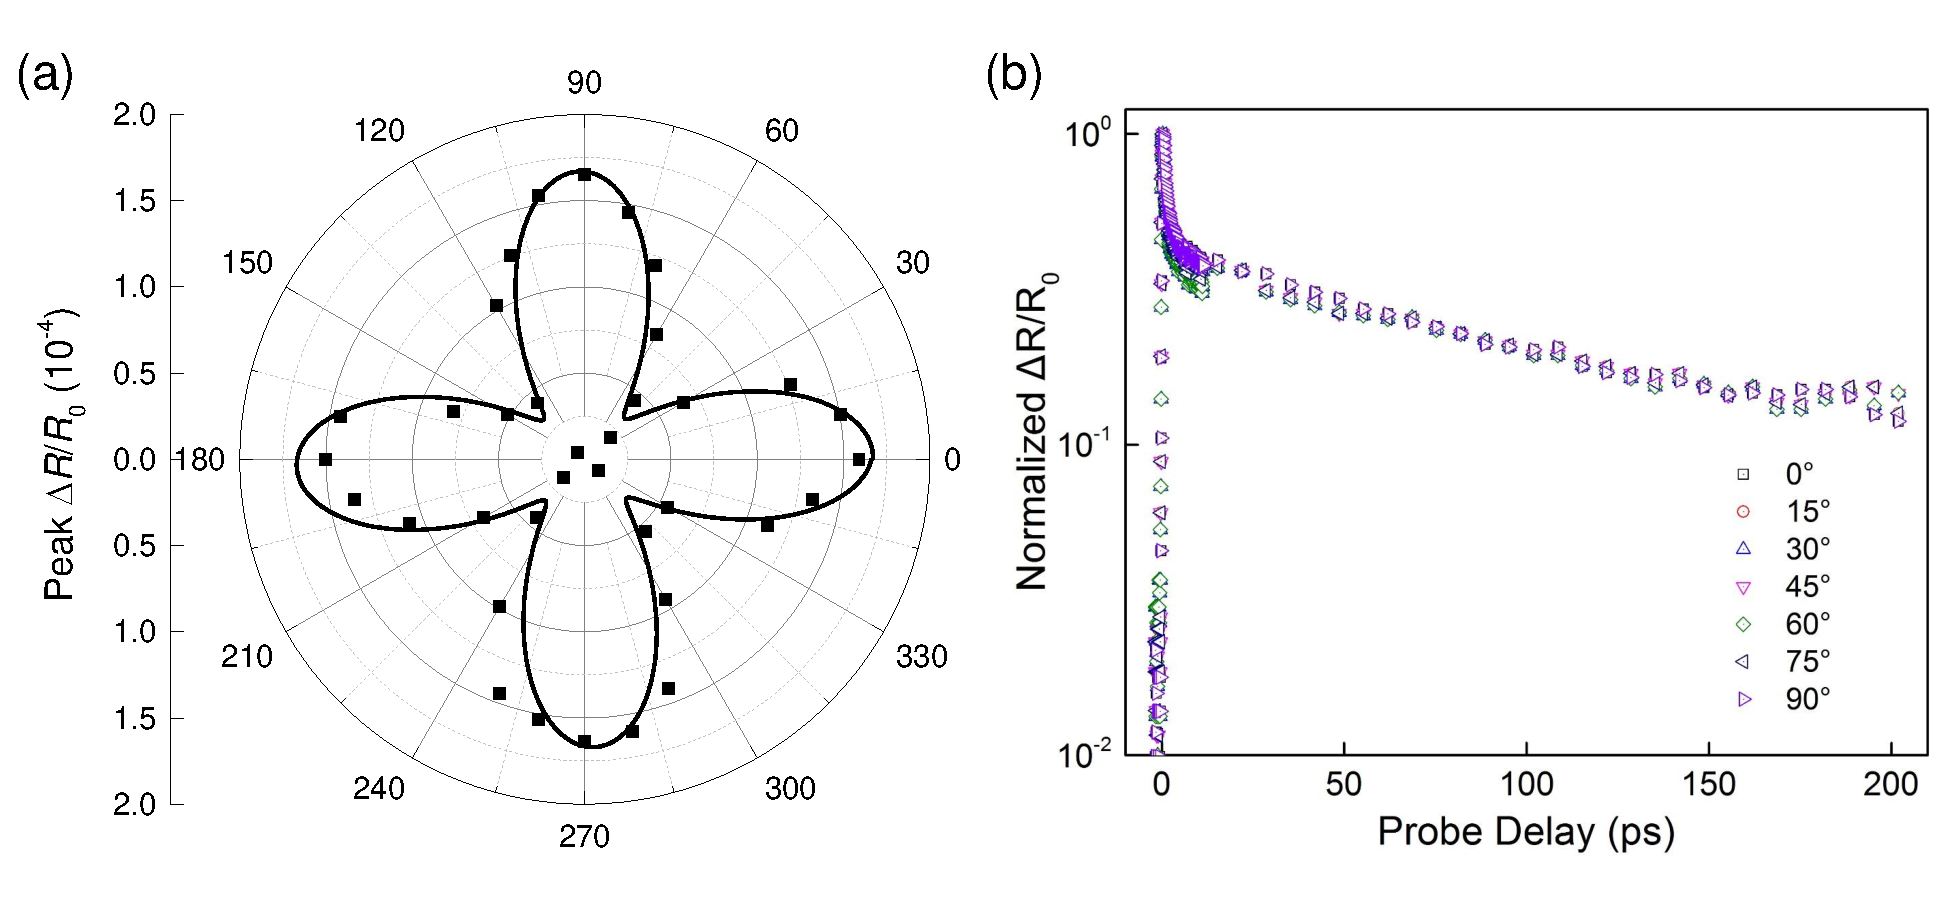
\includegraphics[width=12cm]{angle.pdf}
  \caption{(a) The peak differential reflection signal as a function of the angle $\theta$. (b) Normalized differential reflection signal measured at different values of $\theta$.}
    \label{fig:angle}
\end{figure}

The measurements summarized in Fig. \ref{fig:bulk} were performed with the long edge of the flake along the H direction, which corresponds to $\theta = 0^\circ$. Since ReSe$_2$ has a distorted octahedral (1$T$) crystal structure with triclinic symmetry, it is interesting to probe how the crystal symmetry impacts the differential reflection signal. Fig. \ref{fig:angle}(a) shows the peak differential reflection signal as a function of the sample orientation $\theta$ with respect to the laboratory coordinates, obtained by rotating the sample about its normal direction [see Fig. \ref{fig:sample}(c)]. We found a pronounced angular dependence. The peak signal occurs when the long edge of the sample is either parallel or perpendicular to H. It was known that the absorption coefficient of ReSe$_2$ is the largest when the Re atom chains are along the light polarization. We attribute the 4-fold symmetry to the potential compensation between the maximum absorption coefficient and the minimal transient absorption response along the parallel and perpendicular directions. Despite of the pronounced angular dependence of the magnitude of the signal, its time evolution is independent of the angle. As shown in Fig. \ref{fig:angle}(b), the signal with seven angles, after been normalized, overlap well. Hence, the study of carrier dynamics is not influenced by the anisotropic response of the material.




\begin{figure}
  \centering
  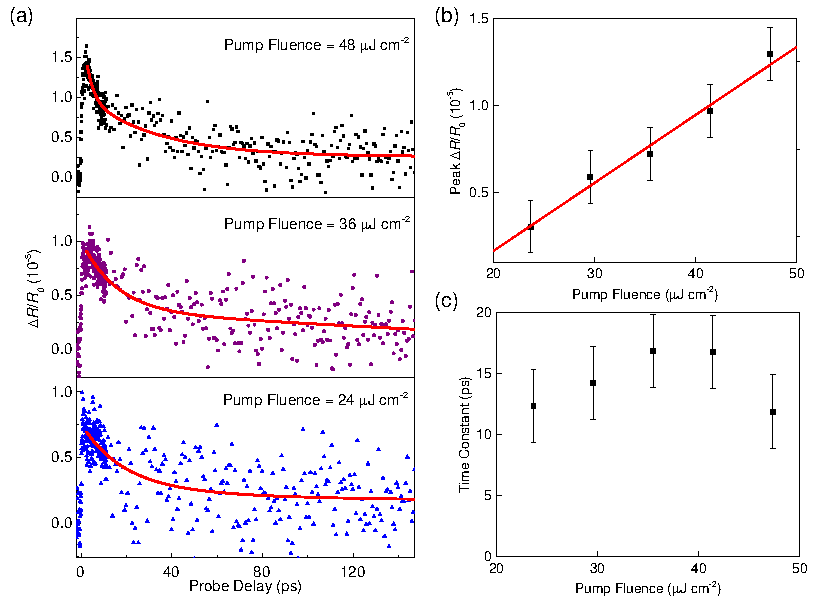
\includegraphics[width=12cm]{ml.pdf}
  \caption{(a) Differential reflection signal measured from a ReSe$_2$ monolayer sample with a 620-nm pump and an 820-nm probe. The solid lines are fits by single-exponential functions. (b) The peak differential reflection signal as a function of the pump fluence. (c) The exponential decay time constant obtained from the fits as a function of the pump fluence.}
    \label{fig:ml}
\end{figure}

We next studied photocarrier dynamics in monolayer ReSe$_2$ with the same technique.  A monolayer ReSe$_2$ film was  fabricated by chemical vapor deposition. The sample was excited by a V-polarized pump pulse of 620-nm, and probed by the 820-nm pulse that is H polarized. Since the sample is a continuous film, the measurement was repeated at multiple randomly selected positions. The results are highly reproducible. Fig. \ref{fig:ml}(a) shows three examples of the obtained signal at different values of pump fluence. A pump fluence of 1 $\mu$J cm$^{-2}$ injects a peak areal carrier density of 3 $\times$ 10$^{10}$ cm$^{-2}$, estimated by using the bulk absorption coefficient \cite{jssc51170}. The signal is much smaller than the bulk sample, due to the reduced sample thickness. Nevertheless, we found that the peak signal is proportional to the pump fluence, as shown in Fig. \ref{fig:ml}(b). We note that due to the low signal-to-noise ratio, fits by bi-exponential is unreliable. We fit the data with a single-exponential function. The obtained decay time constant is plotted in Fig. \ref{fig:ml}(c). We found that the photocarrier lifetime in monolayer ReSe$_2$ is on the order of 10 ps, which is a few times smaller than bulk. Although for the monolayer sample, one would expect similar anisotropic behavior as shown in Fig. \ref{fig:angle}. We could not probe this because the signal from monolayer is too weak and it is difficult to maintain the laser spots on the same crystalline domain when rotating the sample.

\section{Conclusion}
In summary, we have performed the first transient absorption measurement of photocarrier dynamics in ReSe$_2$ bulk and monolayer sample. By measuring differential reflection signals of a 820-nm probe under the excitation of a 620-nm pump, we observed ultrafast thermalization and relaxation of hot carriers in bulk ReSe$_2$. We found that the photocarrier lifetime in bulk ReSe$_2$ is on the order of 80 ps, and decreases slightly with increasing the carrier density. The energy relaxation is also found to be faster at higher densities. Pronounced anisotropic response of transient absorption was observed, however, the carrier dynamics is not influenced by the crystal orientation. Finally, we studied monolayer ReSe$_2$ samples obtained by chemical vapor deposition. We deduced a photocarrier lifetime on the order of 10 ps. These results provide fundamental information for using this material in various optoelectronic devices.

\section*{Funding}

National Key R\&D Program of China
(2016YFA0202302); MOST of China (2016YFA0200602); the National Natural Science Foundation of China (61335006, 61527817, 61378073, 11474260, 11504364); Initiative Postdocs Supporting Program of China (BX201600013); General Financial Grant from the China Postdoctoral Science Foundation (2017M610756); Overseas Expertise Introduction Center for Discipline Innovation, 111 Center of China; National Science Foundation of USA (DMR-1505852).

\end{document}
